\section{Data Gathering Approaches}\label{sec:methods}
In the pursuit of optimizing a program's data locality, implementing visual aids to represent data movements and data layouts can be particularly helpful. This approach enables quick and effective identification of data-related issues, their comprehension, and ultimately, their resolution. This method empowers not only program optimization experts but also domain researchers to effortlessly optimize their programs.

To enable such effective visualization, however, it is essential to first collect information regarding data locality. Several studies have explored this area, leading to the identification of three primary strategies: Dynamic Analysis, Static Analysis, and Simulation. These strategies, which we will delve into in Sections \ref{sec:dynamic_analysis}, \ref{sec:static_analysis}, and \ref{sec:simulation}, each bring their unique benefits and drawbacks. Furthermore, it is important to note that some techniques used for gathering data locality information may not be confined to just one of these three fundamental categories, and could instead exhibit characteristics of multiple approaches.

Once data locality information is gathered, it needs to be presented in a user-friendly manner. There exists a wide variety of visualization techniques that can fulfill this requirement, some of which we will detail in Section \ref{sec:visualization}.

Finally, in Section \ref{sec:optimization_workflow}, we will provide a brief overview of the standard procedure a performance engineer employs to pinpoint memory-related bottlenecks and subsequently enhance the program's data locality.

\subsection{Dynamic Analysis}\label{sec:dynamic_analysis}
Dynamic analysis involves examining a program's data locality by running the program and simultaneously collecting relevant memory-oriented data and statistics. These techniques are widely utilized not only for memory performance analysis, but also to gain a comprehensive understanding of a program's overall performance. Hardware counters, in-built features, are commonly used to measure diverse aspects of a program's execution including the number of cache misses, the number of instructions executed, and the number of floating-point operations performed.

Nevertheless, for effective performance analysis, it is essential to pinpoint the exact location in the source code where bottlenecks occur, such as specific lines of code or function calls. In the absence of this contextual information, discerning the root cause of a performance issue can be challenging. Thus, simply monitoring hardware counters during the program's execution is insufficient. It's equally crucial to track the program's execution flow, so that the hardware counter data can be tied back to the source code. This can, for example, be achieved through the instrumentation of the program's source code with additional instructions that record the program's execution and store performance-related data.

Several prominent techniques for dynamic analysis of a program's data locality are discussed below \cite{shende1999profiling,itzkowitz2003memory,gimenez2017memaxes,mckinley1999quantifying,adhianto2010hpctoolkit}.

Profiling involves periodically interrupting the program's execution to capture both hardware-derived attributes and context-related information \cite{itzkowitz2003memory,gimenez2017memaxes,adhianto2010hpctoolkit}. Profiling techniques analyze the program's call stack and program counter to provide specific details such as the current line of code being executed, the symbol, and, for arrays, the accessed index. This information facilitates the derivation of deeper metrics, such as the number of cache misses per array \cite{adhianto2010hpctoolkit}. Profiling for data locality typically focuses on memory-related events, but the constant interruption can increase runtime overhead. Hence, a trade-off between the granularity and the quality of the measurements is necessary.

Tracing, another technique, allows for a temporal understanding of a program's behavior by logging event-specific data over time. Tracing functions by documenting specific events or functions during program execution, providing a chronological account of these events and their corresponding data. This timeline view of the data contrasts the result that profiling produces, where data is aggregated per instrumented region \cite{shende1999profiling,adhianto2010hpctoolkit,mckinley1999quantifying}.

Profiling and tracing can be implemented through source code instrumentation, recording all pertinent memory accesses. In this way, all relevant memory accesses are recorded. An alternative to instrumentation is statistical sampling, capturing the program's state at regular intervals instead of event-triggered interruptions. The advantage of statistical sampling over instrumentation is that it avoids frequent interruption of the program's execution, reducing the runtime overhead. However, high-quality measurements require sufficiently high sampling rates to capture all relevant details \cite{adhianto2010hpctoolkit}.

In conclusion, dynamic analysis offers several distinct advantages in the study of a program's behavior concerning data locality. As the program is being executed, it offers more precise practical insights into hardware oriented data locality optimization. Further, dynamic analysis can be employed in conjunction with actual data, making it more representative of real-world scenarios.

However, it's important to note the inherent disadvantages of dynamic analysis. The act of running an entire program can be time-consuming and costly, particularly for larger and more complex software. In addition, dissecting specific parts of a program, isolated from the rest, can be rather complex, if not impossible with dynamic analysis. In such cases, other techniques such as static analysis (Section \ref{sec:static_analysis}) may be more applicable.

\subsection{Static Analysis}\label{sec:static_analysis}

Unlike dynamic analysis, static analysis takes a different tack in examining a program's data locality. Instead of operating the program in real-time to gather data, static analysis scrutinizes the program's source code itself. By transforming the source code into an intermediate representation (IR) that centers on data, and subsequently analyzing this IR, static analysis is able to uncover memory-related issues \cite{schaad2022boosting,schaad2021boosting,calotoiu2022lifting,ben2023bridging}.

There are myriad IRs in use, like MLIR \cite{lattner2020mlir}, which are predominantly control-flow oriented, facilitating optimizations pivoting around control elements like loop restructuring \cite{moses2021polygeist}. However, in the context of data locality, data-centric IRs such as SDFG (\cite{ben2019statefulSDFG}), PROGRAPH (\cite{matwin1985prograph}), and LabVIEW (\cite{kodosky2020labview}) provide a more direct approach. By prioritizing memory, its movements, and its computation-induced alterations, these IRs allow for both automated \cite{ben2019statefulSDFG} and, when paired with visual aids, manual enhancements of data locality \cite{ben2023bridging,ben2019statefulSDFG,schaad2021boosting}.

\begin{figure}
  \centering
  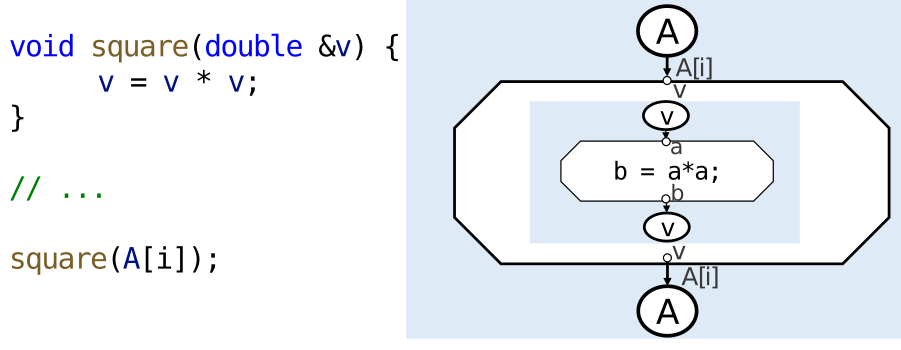
\includegraphics[width=\linewidth]{pictures/SDFG.png}
  \caption{\texttt{C++} language source code and its corresponding SDFG representation \cite{calotoiu2022lifting}.}
  \label{fig:sdfg}
\end{figure}

\begin{figure*}
	\begin{subfigure}[c]{.30\textwidth}
		\centering
		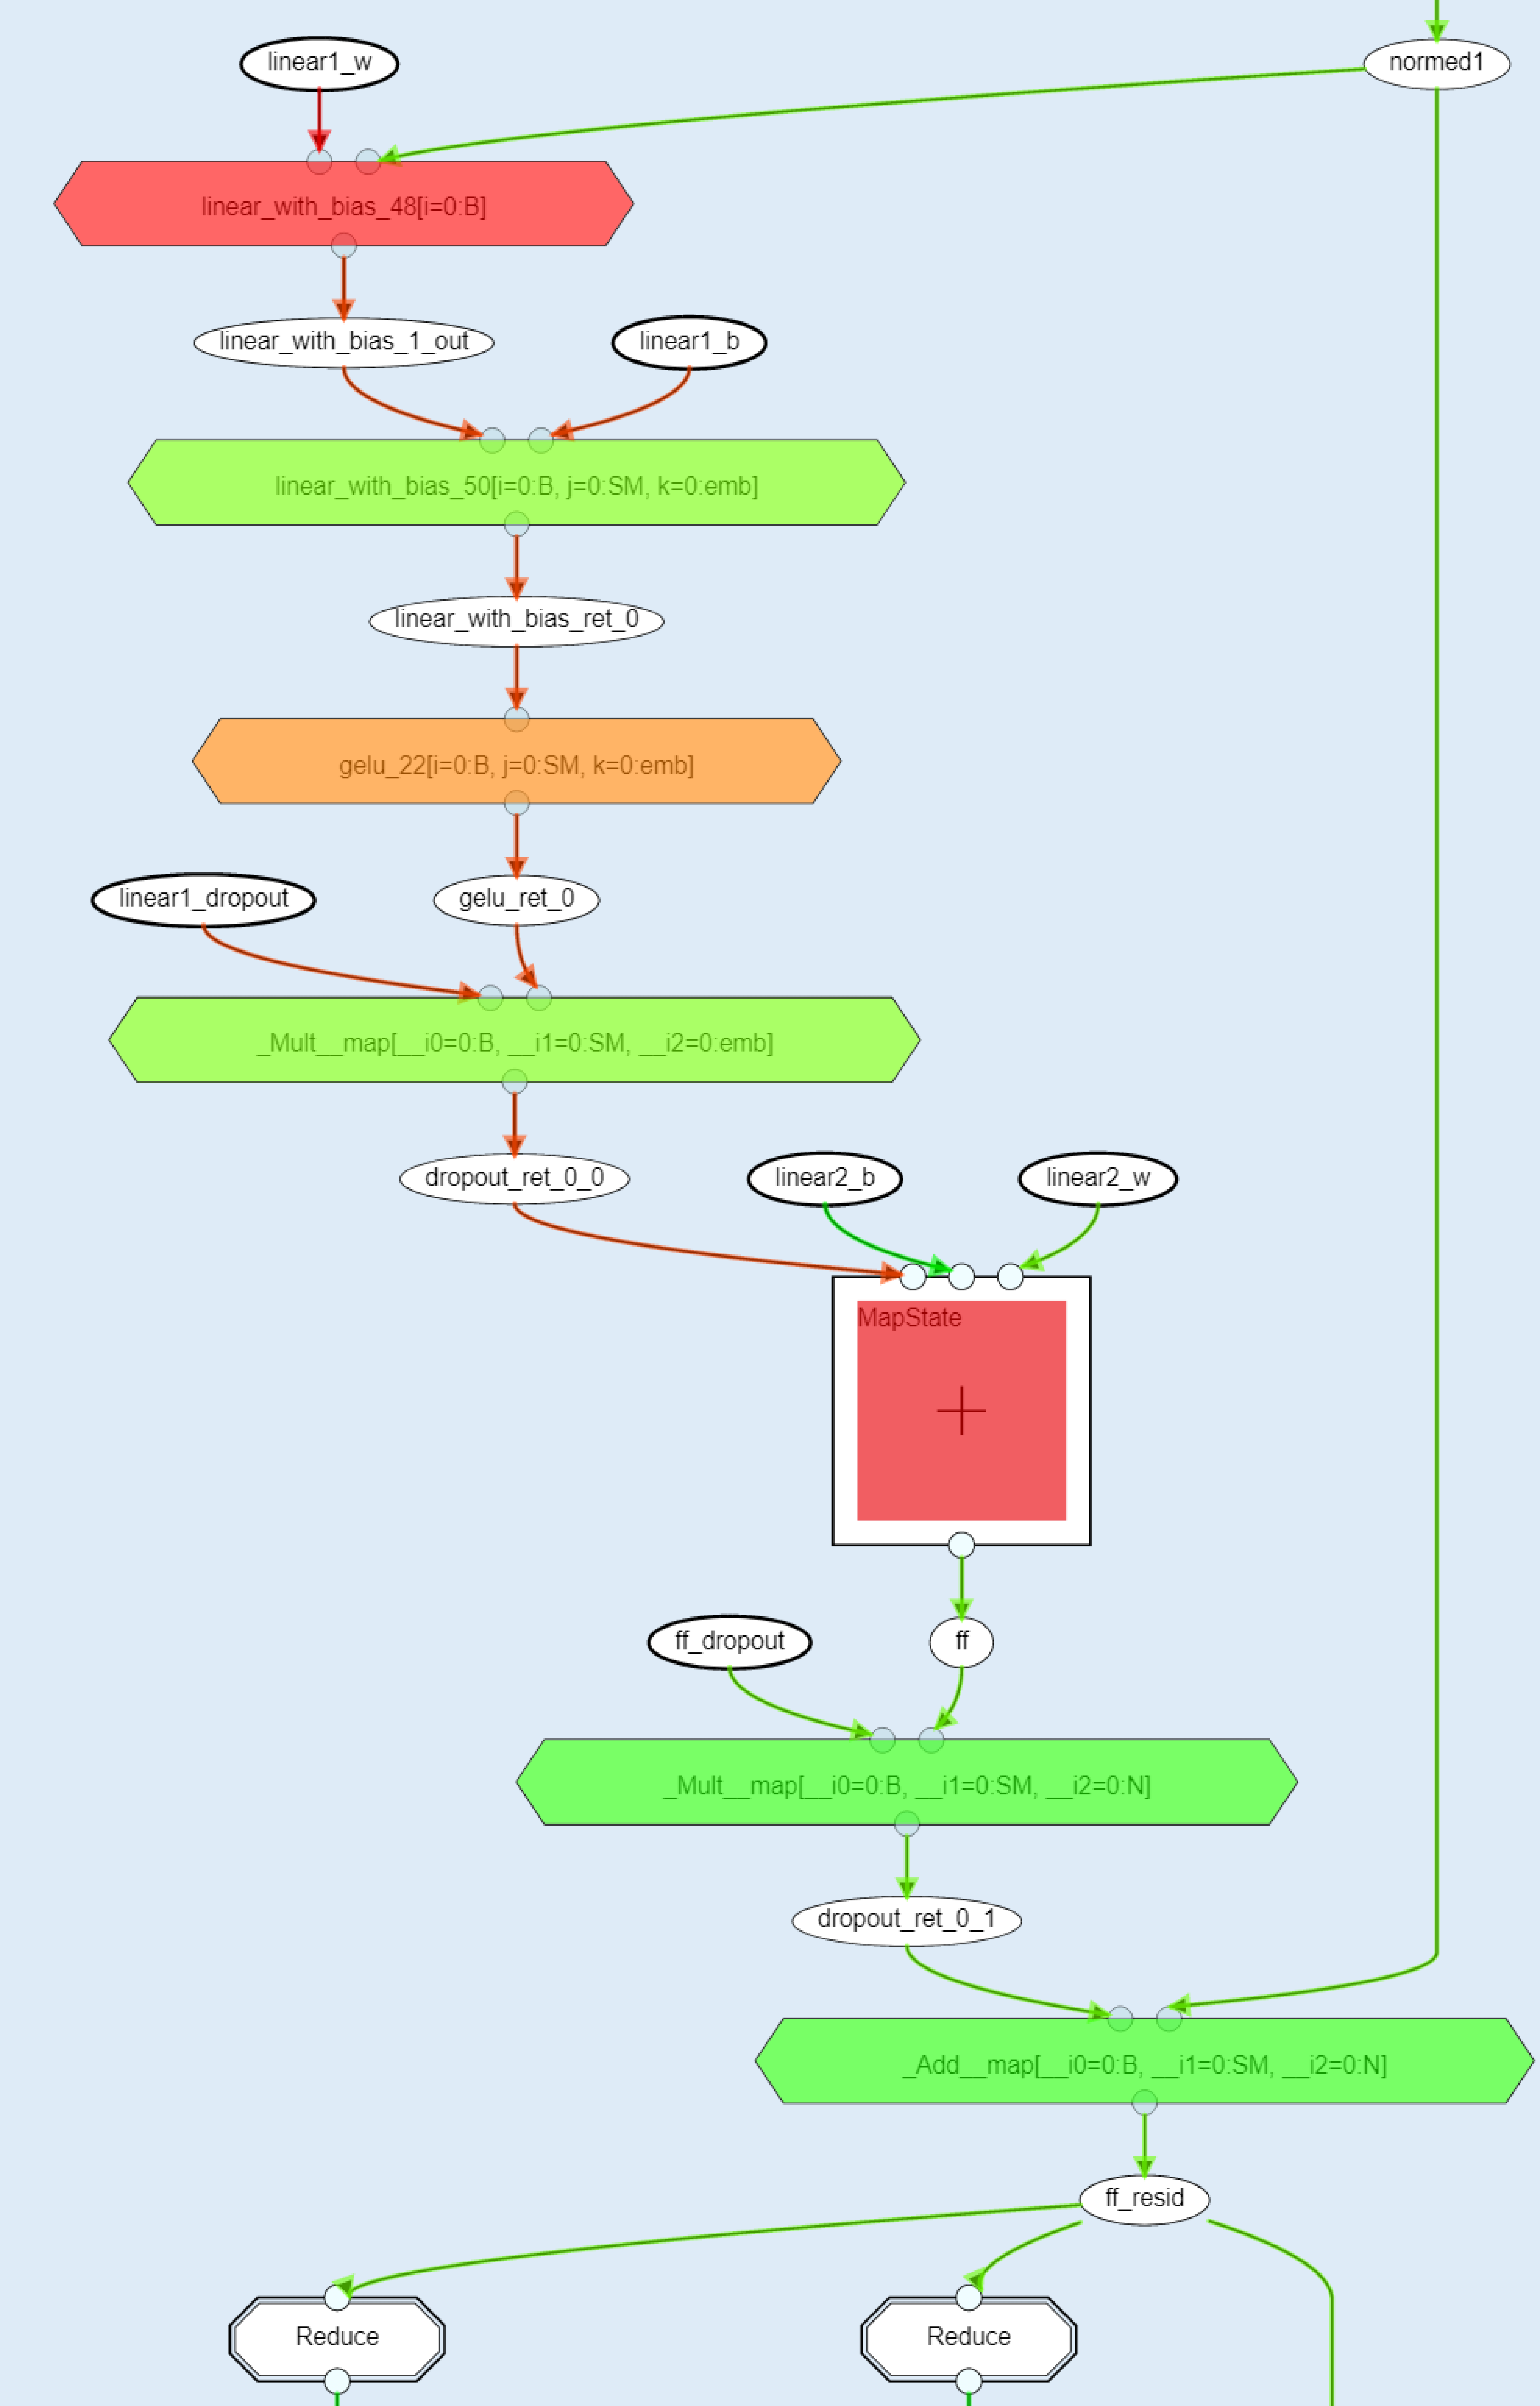
\includegraphics[width=\linewidth]{pictures/boosting_master_both.png}
	\end{subfigure}
	\begin{subfigure}[c]{.68\textwidth}
		\centering
		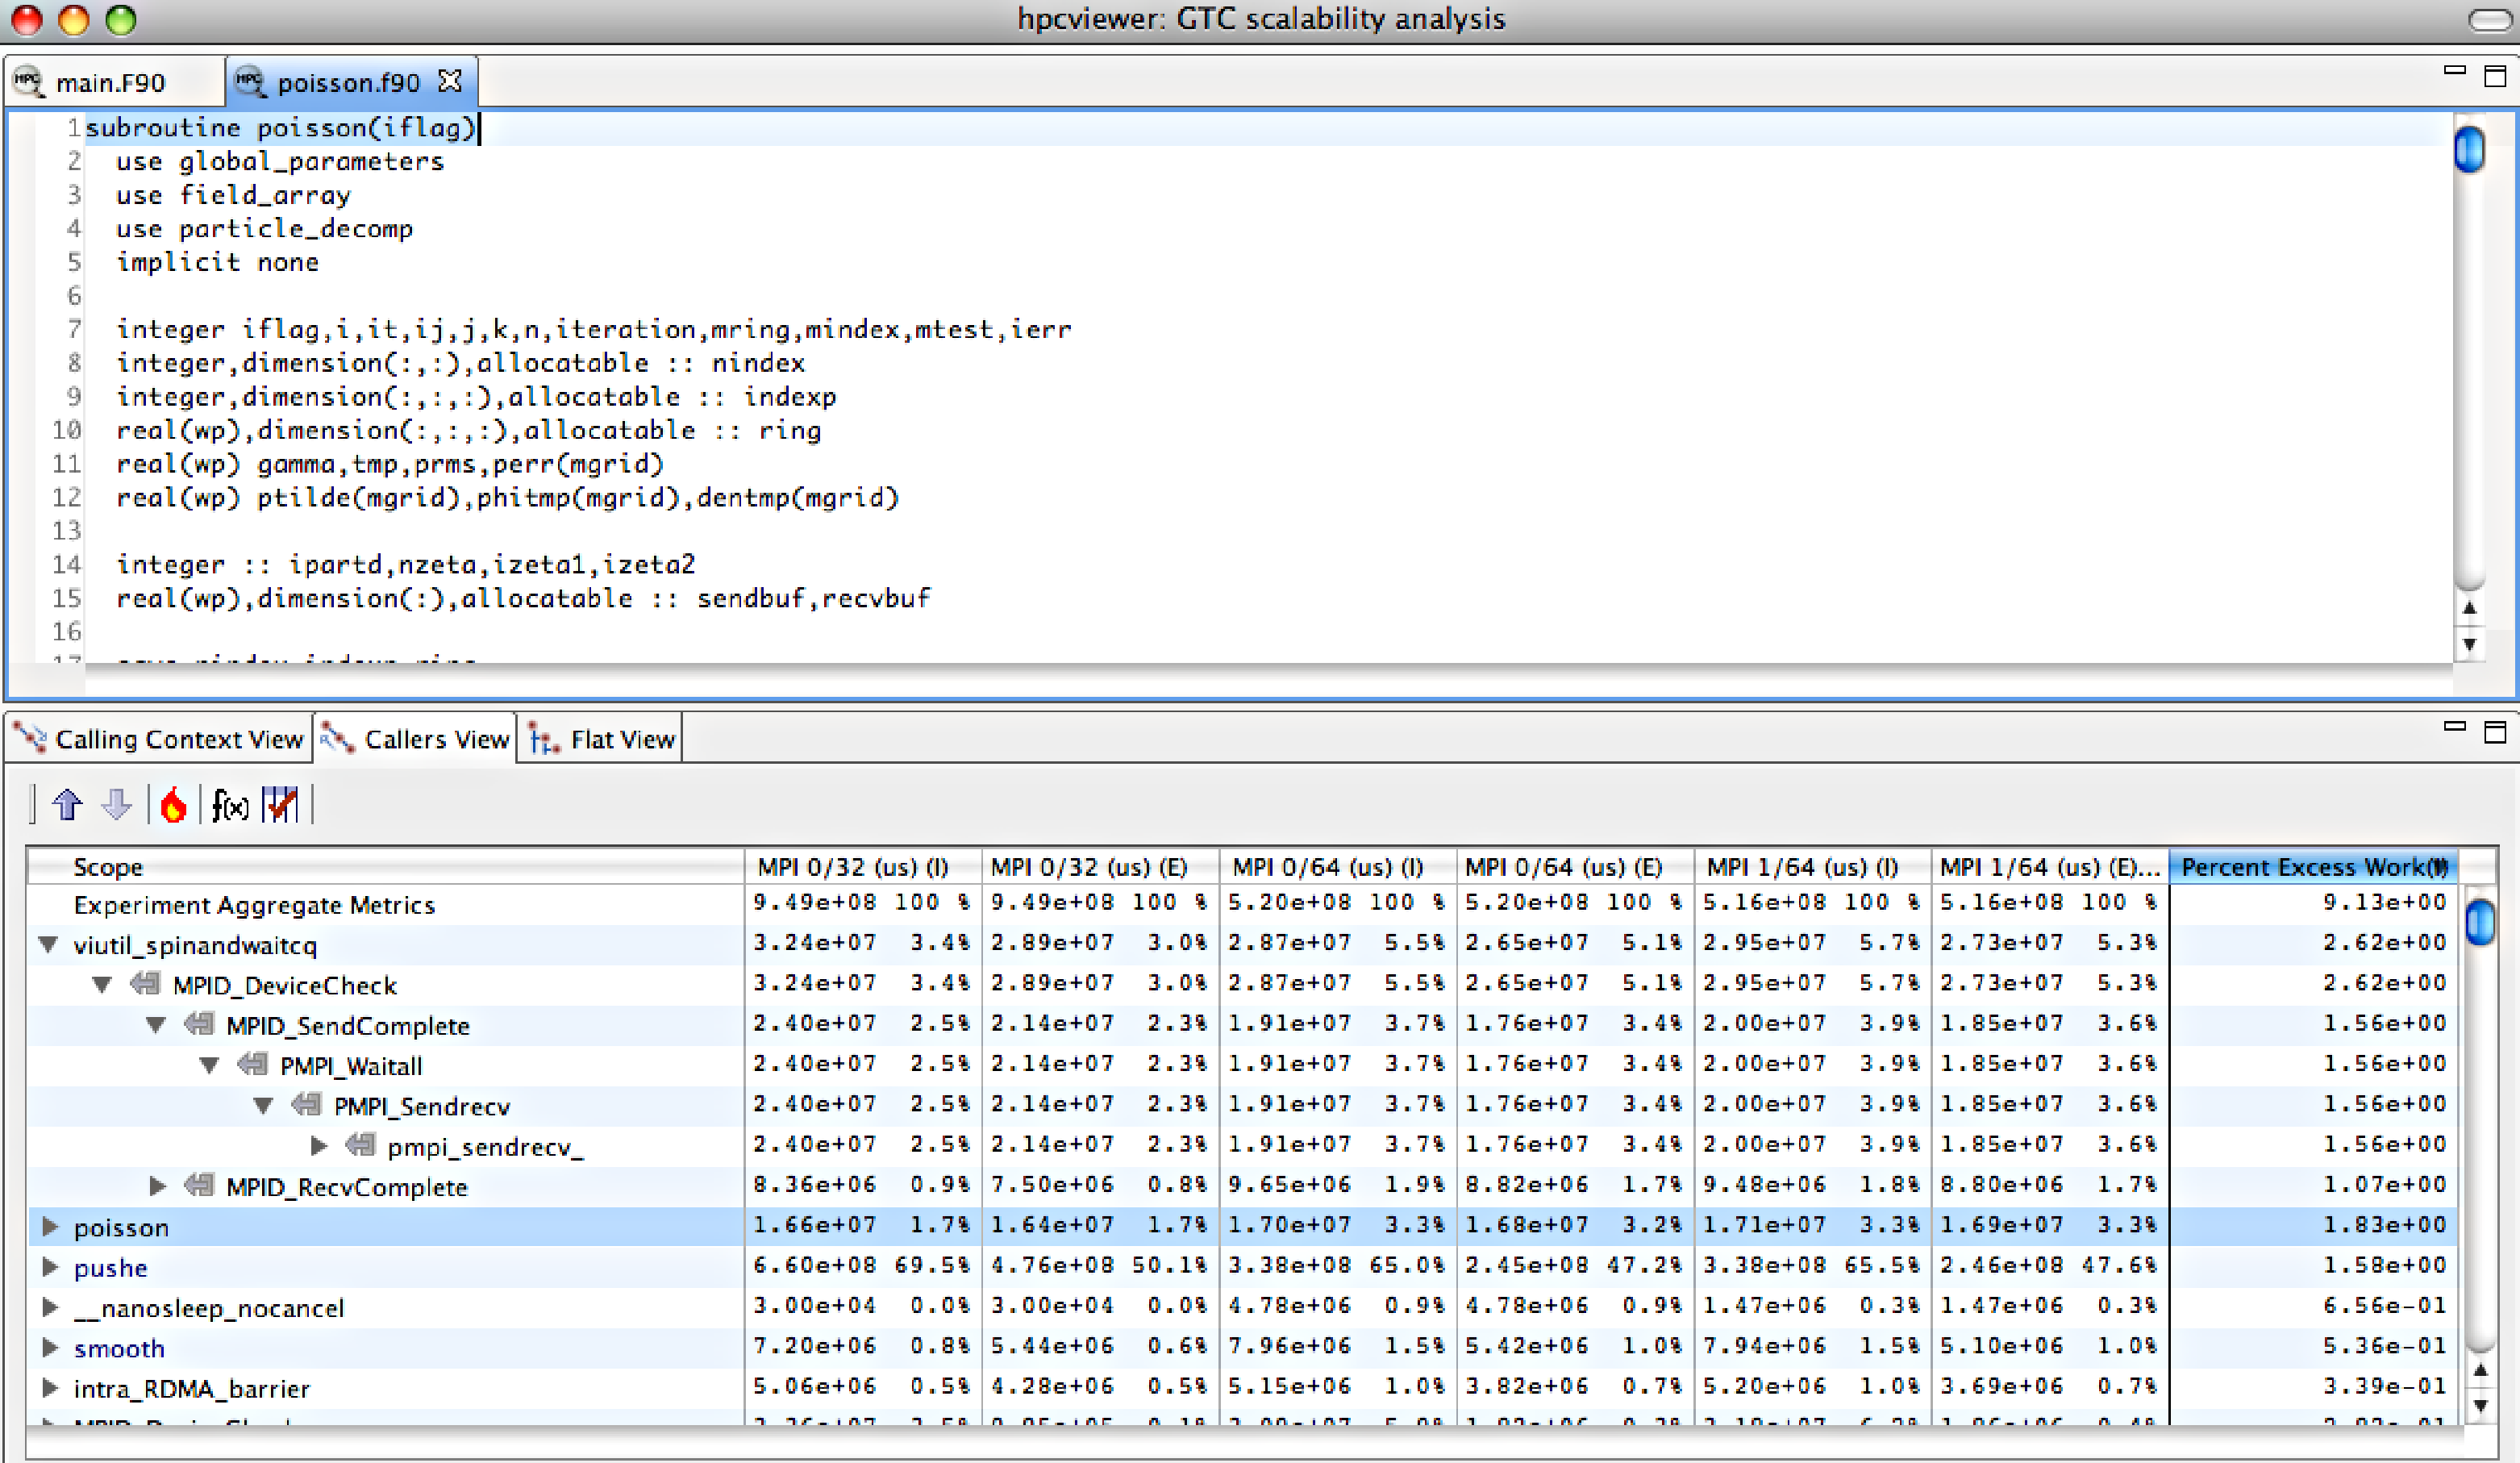
\includegraphics[width=\linewidth]{pictures/hpctoolkitviewer.png}
	\end{subfigure}
	\caption{Left: Coloring in-memory volume onto memlets and arithmetic intensity onto tasklets in an SDFG \cite{schaad2021boosting}. Right: \texttt{HPCToolkit}'s viewer, which displays the program's source code and its corresponding memory access information \cite{adhianto2010hpctoolkit}.}
	\label{fig:coarse}
\end{figure*}

Taking the example of SDFGs, the entire data flow of a program can be represented as a directed graph. Nodes within this graph symbolize $N$-dimensional arrays of data, computations (tasklets), or map scopes that denote general parallelism (such as loops). The edges, or memlets, in an SDFG represent explicit data movements \cite{ben2019statefulSDFG}. An example of the SDFG IR is provided in Figure \ref{fig:sdfg}. Here, the \texttt{square} function found in the source code corresponds to the outer tasklet in the SDFG. The reference \texttt{v} is the sole input and output of this function. This function contains a single computation and assignment \texttt{v = v*v;}, which is translated within the SDFG IR to the tasklet \texttt{b = a*a;}, where \texttt{a} is the input to this computation and \texttt{b} the output. To signify that the value stored in the reference \texttt{v} must be loaded prior and written to following the computation, memlets are used from \texttt{v} to and from the inner tasklet. Ultimately, the method \texttt{square} is invoked, which aligns with loading the parameter \texttt{A[i]} into the reference \texttt{v} and writing the result back to \texttt{A[i]}. In other words, the two tasklets of \texttt{A} from and to the function's tasklet correspond to the loading and writing actions.

As the SDFG IR of a program is constructed, it is possible to compute memory-related properties crucial for data locality. For instance, each memlet carries information regarding the volume of data transported between nodes \cite{ben2019statefulSDFG}, and tasklets and nested SDFGs can be annotated with metadata related to the number of executions and arithmetic operations undertaken \cite{schaad2021boosting}. Consequently, SDFGs offer a comprehensive view of the program and facilitate the identification of data movement bottlenecks on a large scale.

Despite static analysis's robust capability for macroscopic program analysis - a trait shared with dynamic analysis - it does not provide the same level of accuracy in the details. Given that performance bottlenecks are often induced by memory accesses that are tied to physical access patterns and hence are hardware-specific, static analysis alone may not accurately predict, for example, the number of cache misses for a particular function. However, the advantage of static analysis lies in the fact that it does not necessitate program execution, thereby enabling quicker and more cost-effective optimization of logical data movements compared to dynamic analysis.

\subsection{Cache Simulation}\label{sec:simulation}

Positioned between dynamic and static analysis lies the realm of simulation-based approaches, of which cache simulation is particularly noteworthy. Cache simulation is a method used to simulate a program's data accesses on a virtual memory hierarchy model. This process allows for an in-depth examination of both spatial and temporal data locality, as introduced on in Section \ref{sec:data_locality}.

The process of setting up a cache simulator can be divided into two ways:

In the first approach, the program is pseudo-executed without any of its actual computations. This process starts by constructing a virtual memory hierarchy that includes caches, in an optimal scenario fully reconstructing an identical virtual copy of the actual hardware in use. As the program proceeds through its lifecycle, corresponding space is allocated in the simulated memory for each instance of allocation, and reciprocally, space is deallocated as per the program's instructions. The simulator emulates each memory access operation, both read and write, according to how a CPU would handle the task. This entails an initial probe in the L1 cache, followed by a potential cache miss procedure if the required data is absent, as discussed in Section \ref{sec:data_transfer}.

This methodology facilitates a comprehensive and accurate representation of the system's memory hierarchy and its interaction with the computing process \cite{schaad2022boosting,hammer2017kerncraft}.

The second approach uses dynamic analysis (Section \ref{sec:dynamic_analysis}) to generate memory traces. These traces are then rerun through the simulator similarly to the previously described approach. Replaying memory traces enables performance engineers to better understand memory access and management behavior within the program \cite{choudhury2011abstract}.

The deployment of cache simulators extends beyond mere prediction of cache misses. When operated in a step-by-step manner, these tools permit the exploration of data access patterns of a procedure at a granular level. Such detailed inspection can uncover potential enhancements in spatial locality, either through modifications in data layout or access strategies, ultimately contributing to improved performance \cite{schaad2022boosting,hammer2017kerncraft,choudhury2011abstract}.

Moreover, cache simulation enables close-up performance analysis of a program, such as focusing on a single function within the source code or limiting memory traces to a specific functional context.

Despite its advantages, accurate cache simulation demands accurate representation of the target architecture, including aspects like cache hierarchy, cache replacement policy, and cache coherence protocol. Any inaccuracies in these parameters can lead to misleading results, potentially causing optimization attempts to inadvertently degrade the program's data locality. As such, securing the necessary information to build a virtual memory hierarchy, whether automated or utilizing the performance engineer's extensive knowledge of the hardware, is essential for successful performance optimization through cache simulation.

\section{Visualization Techniques}\label{sec:visualization}
\begin{figure}
	\centering
	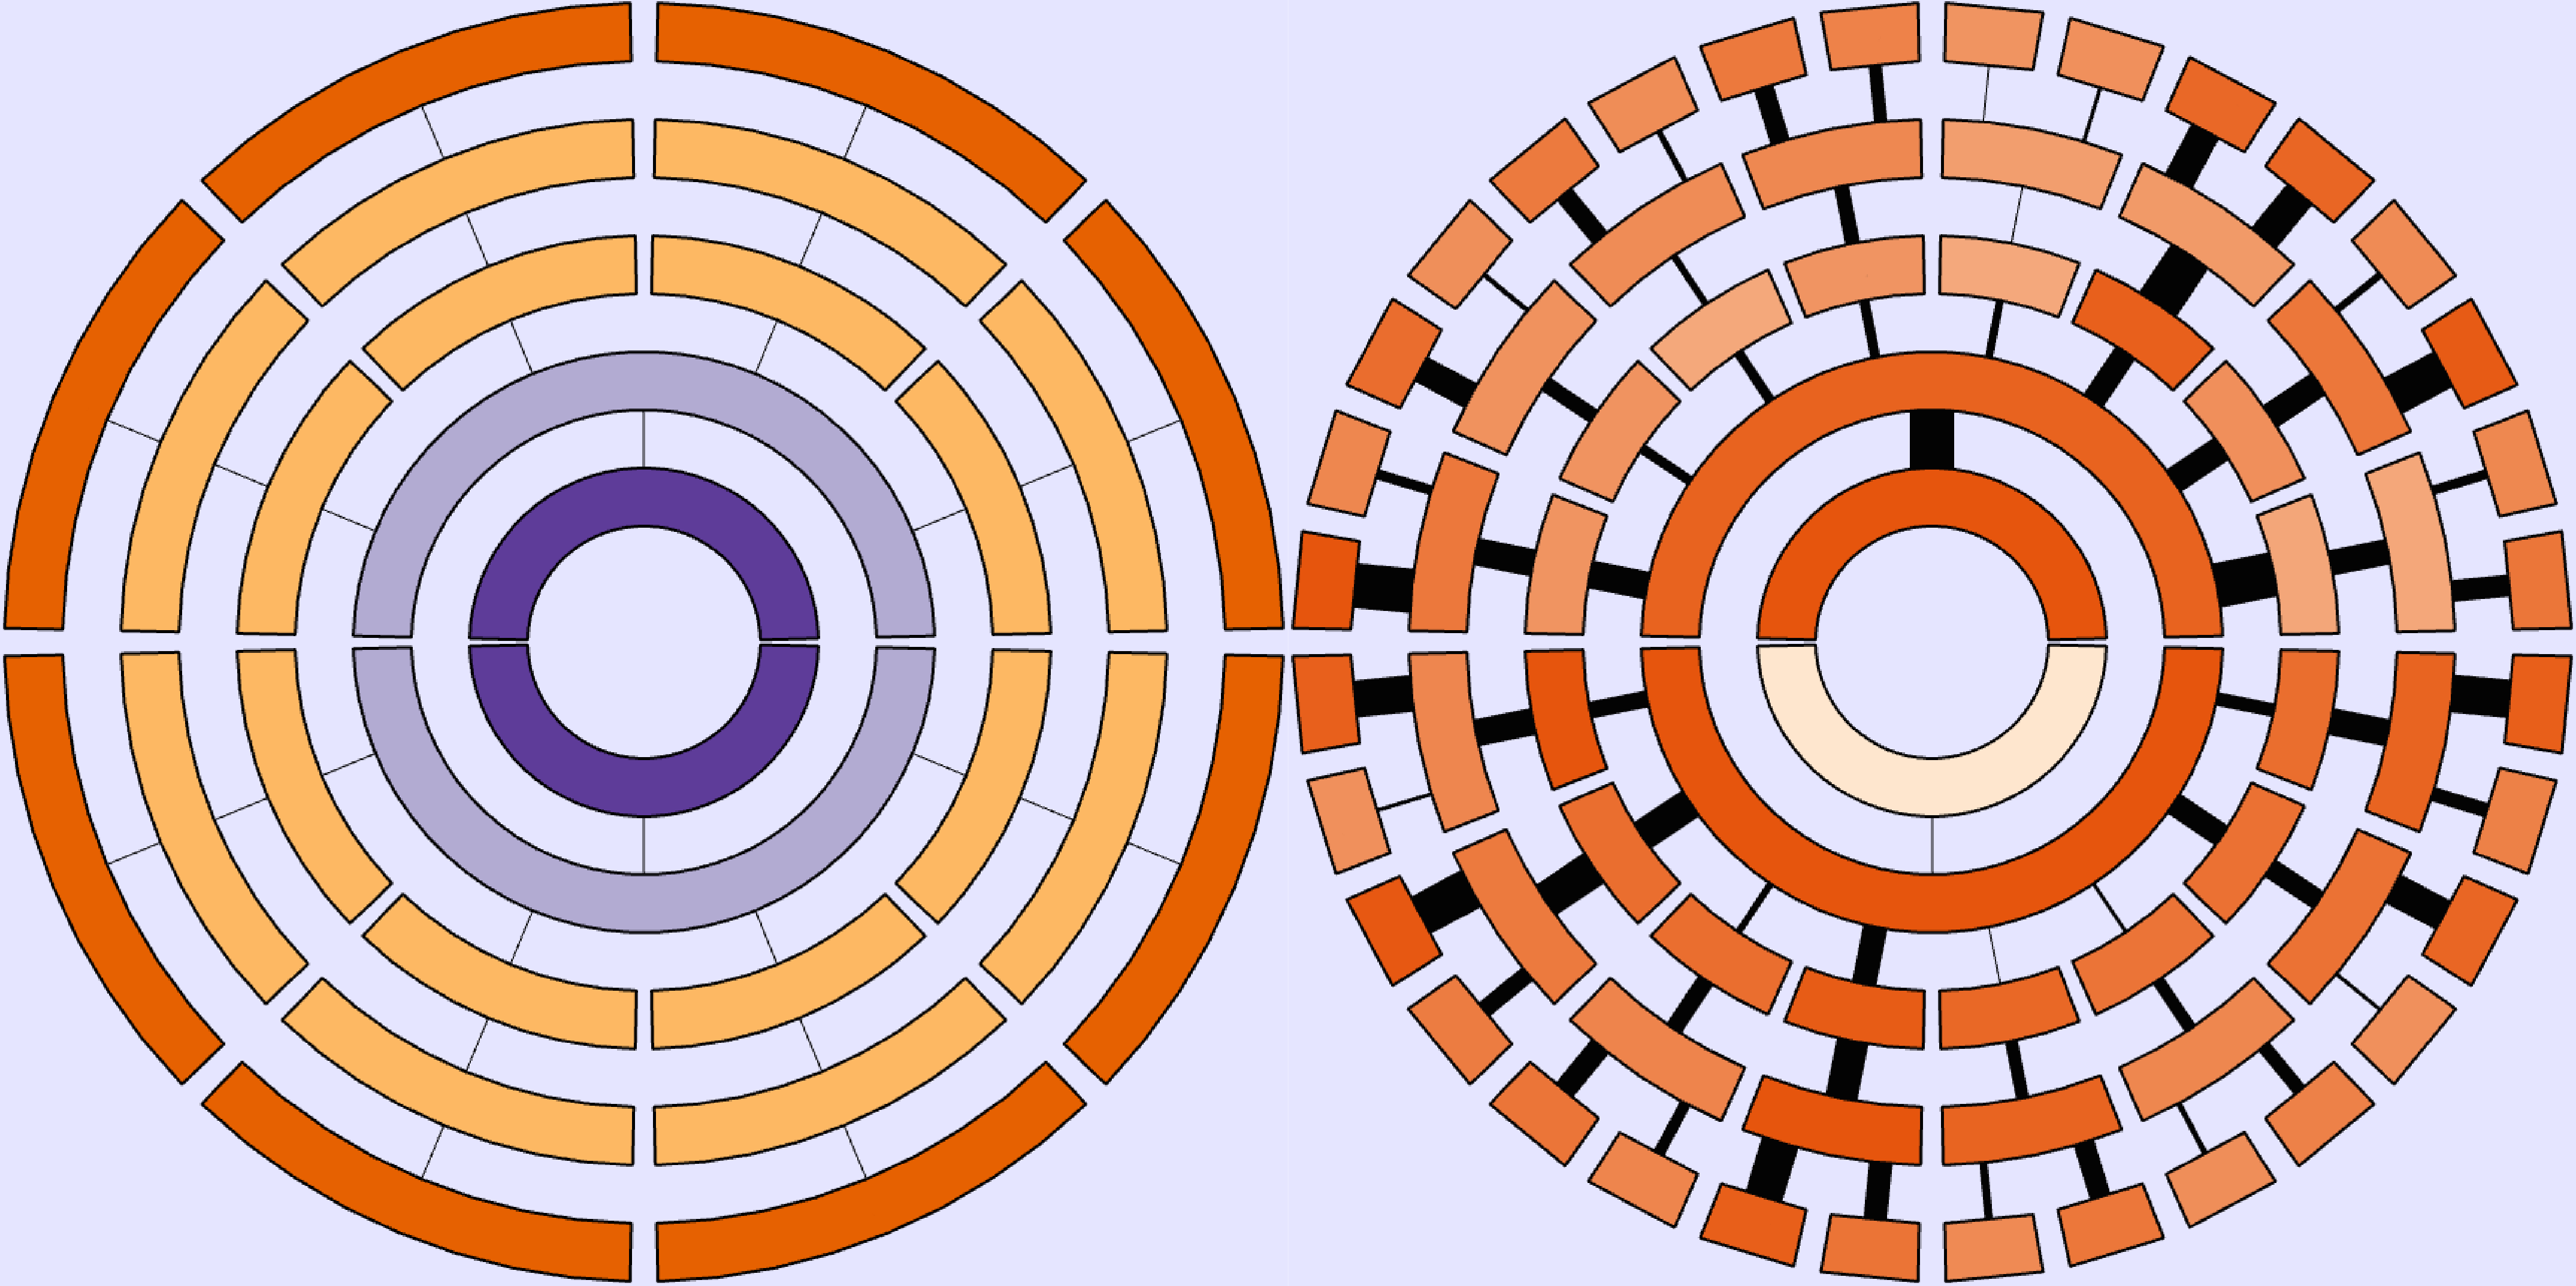
\includegraphics[width=\linewidth]{pictures/memaxes_cache.png}
	\caption{Left: The radial design representing the hardware topology. Main memory resources are depicted in deep purple and processing units in dark orange, with different layers of caches in between. Right: A concrete complex architecture is portrayed based on the radial design on the left, featuring performance data tagged onto the hardware resources through a color code, and transactions among them indicated by line thickness \cite{gimenez2017memaxes}.}
	\label{fig:memaxes_cache}
\end{figure}

Visualization is an essential aspect of data locality analysis, providing the vital link between the analysis results and user comprehension. Effective visualization techniques should balance intuitiveness and informational value. Generally, visualizations for memory-related data can be classified into three categories, each catering to a specific level of detail:

\subsection{High-Level View}\label{sec:coarse_view}
This category of visualization provides the most abstract or "bird's eye" view of data locality, aiming to deliver a global understanding of the program's performance. It emphasizes the logical data movement behavior, spotlighting the performance impact of individual parts of the program \cite{schaad2021boosting,schaad2022boosting,gimenez2017memaxes,adhianto2010hpctoolkit}, as illustrated in Figure \ref{fig:coarse}. The left portion of the figure displays a colored-in SDFG IR of the program, used to demonstrate the arithmetic loads of specific program parts (tasklets), as well as the volume of data circulated throughout the program (memlets). Here, tasklets and memlets marked in red signify above-average intensity, indicating these areas are particularly noteworthy for further exploration concerning performance bottlenecks \cite{schaad2021boosting}. The figure's right side presents a snapshot view of the \texttt{HPCToolkit}'s viewer, wherein performance-related issues can be traced to their source using a hierarchical view of the program's execution \cite{adhianto2010hpctoolkit}. In general, an integral feature of such high-level visualizations is hierarchical clustering, which allows users to zoom into specific areas of the program. Despite providing a broad performance landscape, these visualizations do not shed light on the root causes of identified bottlenecks, warranting a more detailed examination.

\subsection{Intermediate-Level View}\label{sec:medium_view}
At the intermediate level, visualizations offer more detailed insights than high-level overviews, targeting specific segments of the program like functions or loops. One common technique involves displaying the hardware topology to visualize physical data movements across different levels of the memory hierarchy, as well as operational intensity for each memory module, as shown in Figure \ref{fig:memaxes_cache}. This more granular perspective assists in understanding performance bottlenecks and can help identify the most promising optimization opportunities \cite{gimenez2017memaxes,choudhury2011abstract}. Yet, it does not provide information about underlying problematic data layout or access patterns, necessitating a deeper, fine-grained examination.

\begin{figure}
	\centering
	\begin{subfigure}[c]{.54\linewidth}
		\centering
		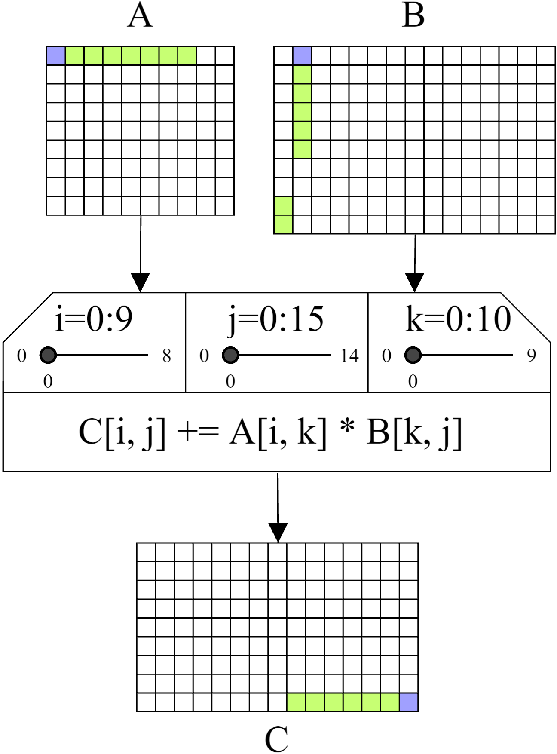
\includegraphics[width=\linewidth]{pictures/boosting_cache_lines.png}
	\end{subfigure}
	\begin{subfigure}[c]{.44\linewidth}
		\centering
		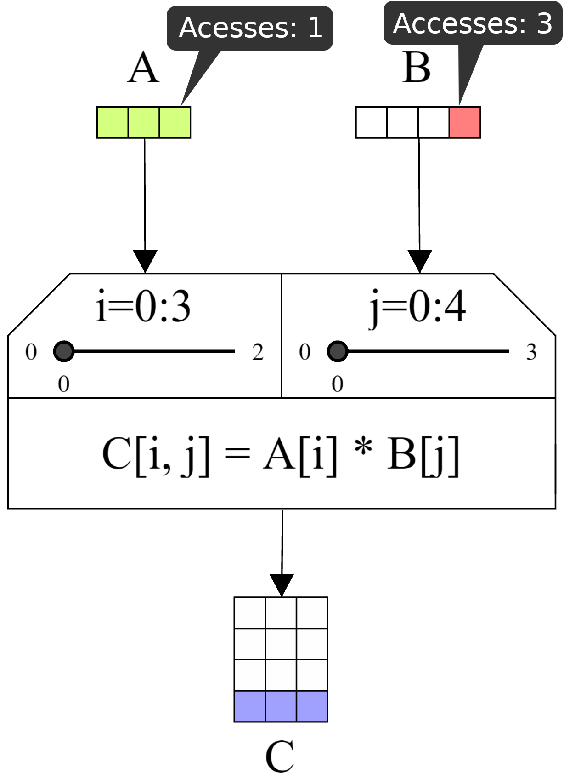
\includegraphics[width=\linewidth]{pictures/boosting_access_patterns.png}
	\end{subfigure}
	\caption{Left: Illustration of data layouts emphasizing spatial locality via cache lines. Right: Visualization of correlated accesses to elements $A$ and $B$ with respect to accesses to $C[3,x], x \in \{0,1,2\}$ \cite{schaad2022boosting}.}
	\label{fig:boosting_cache}
\end{figure}

\subsection{Detailed View}\label{sec:fine_view}
The detailed or fine-grained visualizations delve into specific aspects like data layout and access patterns within specific program segments, for instance, a loop nest. Figure \ref{fig:boosting_cache} displays two examples of such visualizations. The left image illustrates the data layout of a matrix, highlighting the spatial locality of elements within a cache line. The right image presents the access patterns of a loop nest, showing the correlation between accesses to different arrays. This level of visualization aids in identifying potential optimization routes, such as reshaping data to improve spatial locality or reordering the loop to enhance data access patterns \cite{schaad2022boosting}. However, these visualizations provide insights into only one program segment at a time and lack a broader picture of the program's overall data locality. Therefore, it's advisable to use a mix of visualization techniques to obtain a comprehensive understanding of a program's data locality.


\section{Optimization Workflow}\label{sec:optimization_workflow}
In the realm of performance optimization, the workflow that an engineer undertakes unfolds in a progressive manner, moving from a macroscopic to a microscopic examination of a program's performance characteristics. This sequential inspection process serves to identify, understand, and eventually resolve performance bottlenecks, particularly those related to data locality.

The optimization journey commences with a high-level, panoramic view of the program's performance landscape (Section \ref{sec:coarse_view}). This abstracted perspective provides a global understanding of how the program operates, emphasizing performance aspects on a module, function, or code-line level. However, while these coarse-level views may signal where performance issues lie, they often fall short in explaining the "why" behind these issues - the root causes that contribute to elevated memory intensity or the sub-optimal utilization of resources.

For these deeper insights, the engineer transitions to more granular, intermediate-level views (Section \ref{sec:medium_view}). These visualizations elucidate the interactions between particular program components and the memory hierarchy, shedding light on data movements across different cache or memory levels and their impact on performance.

In cases where performance irregularities remain elusive, the engineer resorts to the most detailed, low-level views (Section \ref{sec:fine_view}). These visualizations present a microcosm of data access patterns, offering the necessary detail to pinpoint, understand, and eventually rectify the root causes of performance issues.

This stepwise deepening in focus, from high to intermediate to low-level views, constitutes the typical progression within the performance optimization workflow. However, it is crucial to note that not every tool caters to each level of granularity.

In the following section (Section \ref{sec:works}), we will explore several prominent tools dedicated to visualizing memory movements and accesses. We will discuss their capabilities in data gathering, visualization techniques, and their ability to provide insights at different levels of detail. We will contrast these tools, emphasizing their respective strengths and weaknesses, and the extent to which they support the comprehensive workflow outlined above.